\documentclass[twoside]{book}

% Packages required by doxygen
\usepackage{fixltx2e}
\usepackage{calc}
\usepackage{doxygen}
\usepackage[export]{adjustbox} % also loads graphicx
\usepackage{graphicx}
\usepackage[utf8]{inputenc}
\usepackage{makeidx}
\usepackage{multicol}
\usepackage{multirow}
\PassOptionsToPackage{warn}{textcomp}
\usepackage{textcomp}
\usepackage[nointegrals]{wasysym}
\usepackage[table]{xcolor}

% Font selection
\usepackage[T1]{fontenc}
\usepackage[scaled=.90]{helvet}
\usepackage{courier}
\usepackage{amssymb}
\usepackage{sectsty}
\renewcommand{\familydefault}{\sfdefault}
\allsectionsfont{%
  \fontseries{bc}\selectfont%
  \color{darkgray}%
}
\renewcommand{\DoxyLabelFont}{%
  \fontseries{bc}\selectfont%
  \color{darkgray}%
}
\newcommand{\+}{\discretionary{\mbox{\scriptsize$\hookleftarrow$}}{}{}}

% Page & text layout
\usepackage{geometry}
\geometry{%
  a4paper,%
  top=2.5cm,%
  bottom=2.5cm,%
  left=2.5cm,%
  right=2.5cm%
}
\tolerance=750
\hfuzz=15pt
\hbadness=750
\setlength{\emergencystretch}{15pt}
\setlength{\parindent}{0cm}
\setlength{\parskip}{0.2cm}
\makeatletter
\renewcommand{\paragraph}{%
  \@startsection{paragraph}{4}{0ex}{-1.0ex}{1.0ex}{%
    \normalfont\normalsize\bfseries\SS@parafont%
  }%
}
\renewcommand{\subparagraph}{%
  \@startsection{subparagraph}{5}{0ex}{-1.0ex}{1.0ex}{%
    \normalfont\normalsize\bfseries\SS@subparafont%
  }%
}
\makeatother

% Headers & footers
\usepackage{fancyhdr}
\pagestyle{fancyplain}
\fancyhead[LE]{\fancyplain{}{\bfseries\thepage}}
\fancyhead[CE]{\fancyplain{}{}}
\fancyhead[RE]{\fancyplain{}{\bfseries\leftmark}}
\fancyhead[LO]{\fancyplain{}{\bfseries\rightmark}}
\fancyhead[CO]{\fancyplain{}{}}
\fancyhead[RO]{\fancyplain{}{\bfseries\thepage}}
\fancyfoot[LE]{\fancyplain{}{}}
\fancyfoot[CE]{\fancyplain{}{}}
\fancyfoot[RE]{\fancyplain{}{\bfseries\scriptsize Generated on Wed Oct 7 2015 11\+:12\+:03 for 2048 by Doxygen }}
\fancyfoot[LO]{\fancyplain{}{\bfseries\scriptsize Generated on Wed Oct 7 2015 11\+:12\+:03 for 2048 by Doxygen }}
\fancyfoot[CO]{\fancyplain{}{}}
\fancyfoot[RO]{\fancyplain{}{}}
\renewcommand{\footrulewidth}{0.4pt}
\renewcommand{\chaptermark}[1]{%
  \markboth{#1}{}%
}
\renewcommand{\sectionmark}[1]{%
  \markright{\thesection\ #1}%
}

% Indices & bibliography
\usepackage{natbib}
\usepackage[titles]{tocloft}
\setcounter{tocdepth}{3}
\setcounter{secnumdepth}{5}
\makeindex

% Hyperlinks (required, but should be loaded last)
\usepackage{ifpdf}
\ifpdf
  \usepackage[pdftex,pagebackref=true]{hyperref}
\else
  \usepackage[ps2pdf,pagebackref=true]{hyperref}
\fi
\hypersetup{%
  colorlinks=true,%
  linkcolor=blue,%
  citecolor=blue,%
  unicode%
}

% Custom commands
\newcommand{\clearemptydoublepage}{%
  \newpage{\pagestyle{empty}\cleardoublepage}%
}


%===== C O N T E N T S =====

\begin{document}

% Titlepage & ToC
\hypersetup{pageanchor=false,
             bookmarks=true,
             bookmarksnumbered=true,
             pdfencoding=unicode
            }
\pagenumbering{roman}
\begin{titlepage}
\vspace*{7cm}
\begin{center}%
{\Large 2048 }\\
\vspace*{1cm}
{\large Generated by Doxygen 1.8.10}\\
\vspace*{0.5cm}
{\small Wed Oct 7 2015 11:12:03}\\
\end{center}
\end{titlepage}
\clearemptydoublepage
\tableofcontents
\clearemptydoublepage
\pagenumbering{arabic}
\hypersetup{pageanchor=true}

%--- Begin generated contents ---
\chapter{Hierarchical Index}
\section{Class Hierarchy}
This inheritance list is sorted roughly, but not completely, alphabetically\+:\begin{DoxyCompactList}
\item J\+Panel\begin{DoxyCompactList}
\item \contentsline{section}{com.\+bulenkov.\+game2048.\+Game2048}{\pageref{classcom_1_1bulenkov_1_1game2048_1_1_game2048}}{}
\end{DoxyCompactList}
\end{DoxyCompactList}

\chapter{Class Index}
\section{Class List}
Here are the classes, structs, unions and interfaces with brief descriptions\+:\begin{DoxyCompactList}
\item\contentsline{section}{\hyperlink{classcom_1_1bulenkov_1_1game2048_1_1_game2048}{com.\+bulenkov.\+game2048.\+Game2048} }{\pageref{classcom_1_1bulenkov_1_1game2048_1_1_game2048}}{}
\end{DoxyCompactList}

\chapter{Class Documentation}
\hypertarget{classcom_1_1bulenkov_1_1game2048_1_1_game2048}{}\section{com.\+bulenkov.\+game2048.\+Game2048 Class Reference}
\label{classcom_1_1bulenkov_1_1game2048_1_1_game2048}\index{com.\+bulenkov.\+game2048.\+Game2048@{com.\+bulenkov.\+game2048.\+Game2048}}
Inheritance diagram for com.\+bulenkov.\+game2048.\+Game2048\+:\begin{figure}[H]
\begin{center}
\leavevmode
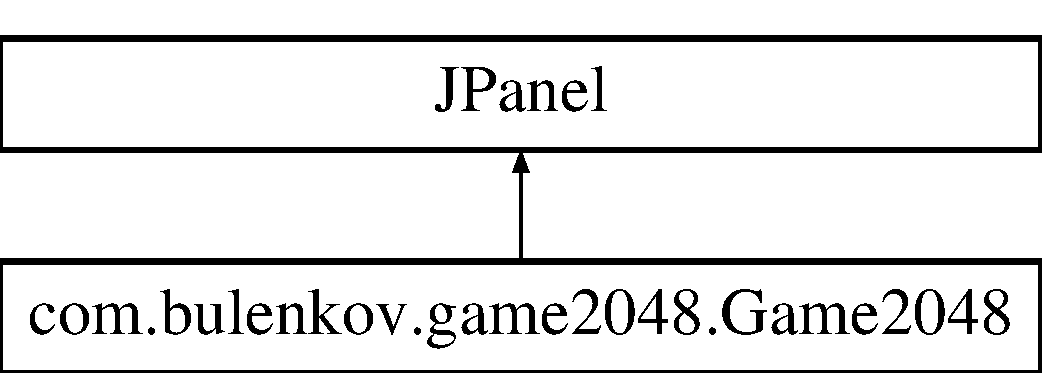
\includegraphics[height=2.000000cm]{classcom_1_1bulenkov_1_1game2048_1_1_game2048}
\end{center}
\end{figure}
\subsection*{Classes}
\begin{DoxyCompactItemize}
\item 
class {\bfseries Tile}
\end{DoxyCompactItemize}
\subsection*{Public Member Functions}
\begin{DoxyCompactItemize}
\item 
\hypertarget{classcom_1_1bulenkov_1_1game2048_1_1_game2048_a6d6f35f0d8bc8f7c794ae32d1d3d0a75}{}void {\bfseries reset\+Game} ()\label{classcom_1_1bulenkov_1_1game2048_1_1_game2048_a6d6f35f0d8bc8f7c794ae32d1d3d0a75}

\item 
\hypertarget{classcom_1_1bulenkov_1_1game2048_1_1_game2048_a5cd88e064d17eadd44a676dc1d27f1c5}{}void {\bfseries left} ()\label{classcom_1_1bulenkov_1_1game2048_1_1_game2048_a5cd88e064d17eadd44a676dc1d27f1c5}

\item 
\hypertarget{classcom_1_1bulenkov_1_1game2048_1_1_game2048_af3f8d3a2c14a4498015feee1d6bfc55b}{}void {\bfseries right} ()\label{classcom_1_1bulenkov_1_1game2048_1_1_game2048_af3f8d3a2c14a4498015feee1d6bfc55b}

\item 
\hypertarget{classcom_1_1bulenkov_1_1game2048_1_1_game2048_aab3725c777a9258dba4d4623fc42668a}{}void {\bfseries up} ()\label{classcom_1_1bulenkov_1_1game2048_1_1_game2048_aab3725c777a9258dba4d4623fc42668a}

\item 
\hypertarget{classcom_1_1bulenkov_1_1game2048_1_1_game2048_aba3585754a10bb682fa3a73b1033f9cb}{}void {\bfseries down} ()\label{classcom_1_1bulenkov_1_1game2048_1_1_game2048_aba3585754a10bb682fa3a73b1033f9cb}

\item 
\hypertarget{classcom_1_1bulenkov_1_1game2048_1_1_game2048_a23c4decbae629c5caf6b7b0f45f46f26}{}void {\bfseries paint} (Graphics g)\label{classcom_1_1bulenkov_1_1game2048_1_1_game2048_a23c4decbae629c5caf6b7b0f45f46f26}

\end{DoxyCompactItemize}
\subsection*{Static Public Member Functions}
\begin{DoxyCompactItemize}
\item 
\hypertarget{classcom_1_1bulenkov_1_1game2048_1_1_game2048_a275a5a0e25aa8838649b6268c03bdb06}{}static void {\bfseries main} (String\mbox{[}$\,$\mbox{]} args)\label{classcom_1_1bulenkov_1_1game2048_1_1_game2048_a275a5a0e25aa8838649b6268c03bdb06}

\end{DoxyCompactItemize}


\subsection{Detailed Description}
\begin{DoxyAuthor}{Author}
Konstantin Bulenkov 
\end{DoxyAuthor}


The documentation for this class was generated from the following file\+:\begin{DoxyCompactItemize}
\item 
2048-\/master/src/com/bulenkov/game2048/Game2048.\+java\end{DoxyCompactItemize}

%--- End generated contents ---

% Index
\backmatter
\newpage
\phantomsection
\clearemptydoublepage
\addcontentsline{toc}{chapter}{Index}
\printindex

\end{document}
